\documentclass[10pt,a4paper]{ULBreport}
\usepackage[utf8]{inputenc}
\sceau{pic/official_logos/sceauULB.png}
\graphicspath{ {./pic/} }
\usepackage{multirow}
\usepackage{listings}
\usepackage{color} 
\usepackage{setspace} 
\usepackage{amsmath}
\usepackage{mathrsfs}
\usepackage{bm}
\usepackage[mathscr]{eucal}
\usepackage{hyperref}
\usepackage{pdfpages}
\usepackage{biblatex}
\usepackage{floatrow}
\usepackage{subcaption} 
\usepackage{siunitx}
\usepackage[many]{tcolorbox}
\usepackage{multirow}
\usepackage{listings}
\usepackage[dvipsnames]{xcolor}
\usepackage{fancyvrb}
\usepackage{graphicx}

\usepackage{xstring}
\usepackage{etoolbox}

% Colors



\begin{document} 


	\titleULB{
	title={V2V communication project},
    studies={M1-IRELE},
    course ={ELEC-H415 Communication Channels},
    author={\textit{Author :} \\ Colot Emmeran },
    date={\textbf{Academic year :} \\ 2024 - 2025},
    teacher={\textit{Professor : } \\ De Doncker Philippe},
    logo={pic/official_logos/logos.jpg},
    manyAuthor
	}

%\listoftables % ToC for tables

%\listoffigures % ToC for figures

\chapter{Introduction}

\begin{center}
    
    \Huge TODO\\
    \vspace{0.5cm}
    \large Might want to check all 3d plots names\\
    Write an introduction
    \normalsize
    
\end{center}
\chapter{Theoretical answers}

\section{Step 1}

\begin{figure}[H]
    \centering
    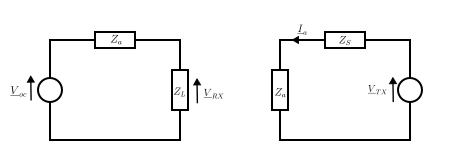
\includegraphics[width=1\textwidth]{circuit.png}
    \caption{Equivalent electric circuit of an antenna in RX (left) and TX (right)}
    \label{fig:equivalent_electrical_circuit}
\end{figure}

Fig \ref{fig:equivalent_electrical_circuit} shows the equivalent electrical circuit at RX and TX where $\underline{V}_{oc}$ is the induced voltage, $\underline{V}_{RX}$ the voltage at the output of the RX antenna, $\underline{V}_{TX}$ at the input of the TX antenna and $\underline{I}_{a}$ the current entering the TX antenna.\\

As both transmitting and receiving antenna are vertical $\lambda/2$ dipoles, their equivalent heights can be analytically computed:

\begin{align*}
    \vec{h}_e (\theta, \phi) = \frac{\lambda}{\pi} \frac{\cos(\frac{1}{2}\cos \theta)}{\sin ^2 \theta}\vec{1_z}\\
    \vec{h}_{e\perp} (\theta, \phi) = -\frac{\lambda}{\pi} \frac{\cos(\frac{\pi}{2}\cos \theta)}{\sin \theta}\vec{1_\theta}
\end{align*}

As $\theta$ and $\phi$ are spherical coordinates, the horizontal plane (in which the simulation is done) corresponds to $\theta = \pi/2$. The transverse equivalent height is then reduced to hte following, where it does not depend on the azimuthal angle $\phi$:

\begin{align*}
    \vec{h}_{e\perp} (\phi) = -\frac{\lambda}{\pi} \vec{1_{\theta}}\\
\end{align*}

The transverse part of the equivalent height gives rise to an expression for the emitted electric field.

\begin{align*}
    \underline{\vec{E}} &= -j\omega \underline{I}_a \frac{\mu_0}{4\pi}\frac{e^{-j\beta r}}{r}\vec{h}_{e\perp}(\theta, \phi) \\
    &= j\omega \underline{I}_a \frac{\mu_0\lambda}{4\pi^2}\frac{e^{-j\beta r}}{r} \vec{1_{\theta}} \\
    &= j \frac{\underline{I}_a \mu_0 c}{2\pi} \frac{e^{-j\beta r}}{r} \vec{1_{\theta}}\\
    &= j \frac{\underline{I}_a Z_0}{2\pi} \frac{e^{-j\beta r}}{r} \vec{1_{\theta}}
\end{align*}

To make the transmission parameters appear in the electric field expression, $\beta$ and $\underline{I}_a$ must be replaced with the formulas given below. $Z_0$, $Z_a$, $Z_S$ can also be replaced by respectively $120\pi$, $\frac{720\pi}{32}$ and $\frac{720\pi}{32}$ (assuming the impedances are matching).

\begin{gather*}
    \beta = \frac{2\pi f_c}{c}\\
    \underline{V}_{TX} = (Z_a + Z_S) \underline{I}_a = \frac{720\pi}{16} \underline{I}_a
\end{gather*}

Wich yields

\begin{align*}
    \underline{\vec{E}} &= j \frac{120\pi\underline{I}_a}{2\pi} \frac{e^{-\frac{j2\pi f_c r}{c}}}{r} \vec{1_{\theta}}\\
    &= j \frac{4\underline{V}_{TX}}{3\pi} \frac{e^{-\frac{j2\pi f_c r}{c}}}{r} \vec{1_{\theta}}
\end{align*}

The last step is to replace the travel distance $r$ with $c \tau$ as the wave is propagating at the speed of light in free space. The electric field thus becomes:

\begin{align*}
    \underline{\vec{E}} &= j \frac{4 \underline{V}_{TX}}{3\pi} \frac{e^{-j2\pi f_c \tau}}{c\tau} \vec{1_{\theta}}
\end{align*}

The voltage at the output of the antenna $\underline{V}_{RX}$ can be deduced from the equivalent electric circuit \ref{fig:equivalent_electrical_circuit} as it is a simple voltage divider. Assuming a matching between the antenna and the load, we have:

\begin{align*}
    \underline{V}_{RX} = \frac{Z_L}{Z_a + Z_L} \underline{V}_{oc} = \frac{1}{2} \underline{V}_{oc}\\
    \underline{V}_{oc} = -\left . \vec{h}_{e\perp}(\theta, \phi)\right\vert_{\theta = \pi/2} \cdot \underline{\vec{E}}_i
\end{align*}

Where $\underline{\vec{E}}_i = - \underline{\vec{E}}$ due to the change of coordinates origin. It is here assumed that there was no reflexion, refraction or transmission through another material. This results in:

\begin{align*}
    \underline{V}_{oc} &= \frac{\lambda}{\pi} \cdot \underline{E}_i\\
    &= -j\frac{4  \lambda \underline{V}_{TX}}{3\pi^2}\frac{e^{-j 2\pi f_c \tau}}{c\tau}\\
    \underline{V}_{RX} &= -j\frac{2  \lambda }{3\pi^2}\frac{e^{-j 2\pi f_c \tau}}{c\tau}\underline{V}_{TX}
\end{align*}

For a practical use in step 3, the time of flight $\tau$ is replaced by the traveled distance $d$ to get:

\begin{align}
    \underline{V}_{RX} &= -j\frac{2 \lambda }{3\pi^2}\frac{e^{-j\frac{2\pi f_c d}{c}}}{d}\underline{V}_{TX}
    \label{eq:voltage_RX}
\end{align}

\section{Step 2}

Assuming the communication takes place via a LOS ray only, the channel impulse response $h(\tau)$ is defined as follows:

\begin{align*}
    h(\tau) = \frac{\alpha_1 e^{-j\frac{2\pi f_cd_1}{c}}}{d_1} \delta(\tau - \frac{d_1}{c})
\end{align*}

Where $d_1$ the distance of propagation of the direct ray. $\alpha_1$ (which might be complex) takes into account a phase change or attenuation due for example to reflections whereas the imaginary exponential next to it corresponds to the phase change due to the propagation delay. In the case of LOS transmission $\alpha_1$ is equal to 1.\\
The transfer function $H(f)$ of the channel is found by taking the Fourier transform of $h(\tau)$

\begin{align*}
    H(f) &= \int_{-\infty}^{\infty} h(\tau) e^{-j2\pi f \tau} d\tau\\
    &= \frac{e^{-j\frac{2\pi f_c d_1}{c}}}{d_1}e^{-j2\pi f \frac{d_1}{c}}\\
    &= \frac{e^{-j \frac{2\pi (f+f_c)d_1}{c}}}{d_1}\\
\end{align*}

As we consider a single ray, the narrowband model of the channel $h_{NB}$ (representing the case where the receiver perceives the sum of all propagation path) is simply found by removing the Dirac pulse from $h(\tau)$

\begin{align*}
    h_{NB} = \frac{e^{-j \frac{2\pi f_cd_1}{c}}}{d_1}
\end{align*}

The ratio between the received power $P_{RX}$ and the transmitted power $P_{TX}$ is found with:

\begin{align}
    \frac{P_{\text{received}}}{P_{\text{transmitted}}} &= \frac{\left| h(\tau) \right|^2}{2} \nonumber\\
    &= \frac{1}{d_1^2}
    \label{eq:power_approx}
\end{align}

This result can be compared with the Friis formula, given by:

\begin{align}
    P_{RX}(d) = P_{TX} G_{TX}(\theta_{TX}, \phi_{TX})G_{RX}(\theta_{RX}, \phi_{RX})\left(\frac{\lambda}{4\pi d}\right)^2
    \label{eq:friis_formula}
\end{align}

The reason for the big difference between the two formulas can be easily explained: in eq \ref{eq:power_approx}, $P_{\text{transmitted}}$ and $P_{\text{received}}$ are the powers of the waves, not the one of the signal before/after passing through the antennas. To correct it, they are replaced by the Poynting vectors $\bm{\vec{\mathscr{S}}}_{TX}$ and $\bm{\vec{\mathscr{S}}}_{RX}$:

\begin{align}
    \frac{\left|\bm{\vec{\mathscr{S}}}_{RX}\right|}{\left|\bm{\vec{\mathscr{S}}}_{TX}\right|} = \frac{1}{d_1^2}
    \label{eq:poynting}
\end{align}

To compare the received and the injected power, the Poynting vectors should be replaced by

\begin{align*}
    \left|\bm{\vec{\mathscr{S}}}_{TX}\right| = G_{TX} P_{TX}\\
    \left|\bm{\vec{\mathscr{S}}}_{RX}\right| A_{eRX} = P_{RX}\\
    \text{where} \quad \quad A_{eRX} = G_{RX}\left(\frac{\lambda}{4\pi}\right)^2
\end{align*}

When placed back in eq \ref{eq:poynting}, the expression matches the Friis formula (eq \ref{eq:friis_formula}). \\
To further simplify and as the antennas are considered to be lossless dipoles, equation \ref{eq:power_friis_simplified} replaces their gain by $\frac{16}{3\pi}$, the theoretical gain of such antennas.

\begin{align}
    \frac{P_{RX}}{P_{TX}} &= G_{TX} G_{RX} \left(\frac{\lambda}{4\pi d_1}\right)^2\\
    \label{eq:power_friis_simplified}
    &= \frac{16}{9\pi^2} \left(\frac{\lambda}{\pi d_1}\right)^2
\end{align}

Two deductions can be made of this result: 
\begin{itemize}
    \item The power loss on the channel depends on the square of the distance between the emitter and the receiver. It implies that doubling the range of an antenna would need a multiplication of the transmitting power by a factor 4.
    \item A more surprising result is the wavelength squared appearing at the numerator. It shows that there is always a compromise between data rate and power consumption as a larger wavelength will indeed be less attenuated but the maximal data rate will then be lowered in order for the channel to still be considered as narrowband.
\end{itemize}

\section{Step 3}

After having implemented a raytracing algorithm, the simulation is able to compute every path from the transmitter to the receiver. Figure \ref{fig:raytracingDemo} shows the result of the simulation for cars spaced by 100m on a 20m wide road surrounded by buildings. For a better understanding, the angles are computed between the buildings and the rays. This is only done on this graph as the angles used to compute the reflection coefficients $\Gamma_{\perp}$ are the ones between the normal to the obstacle and the ray.

\begin{figure}[H]
    \centering
    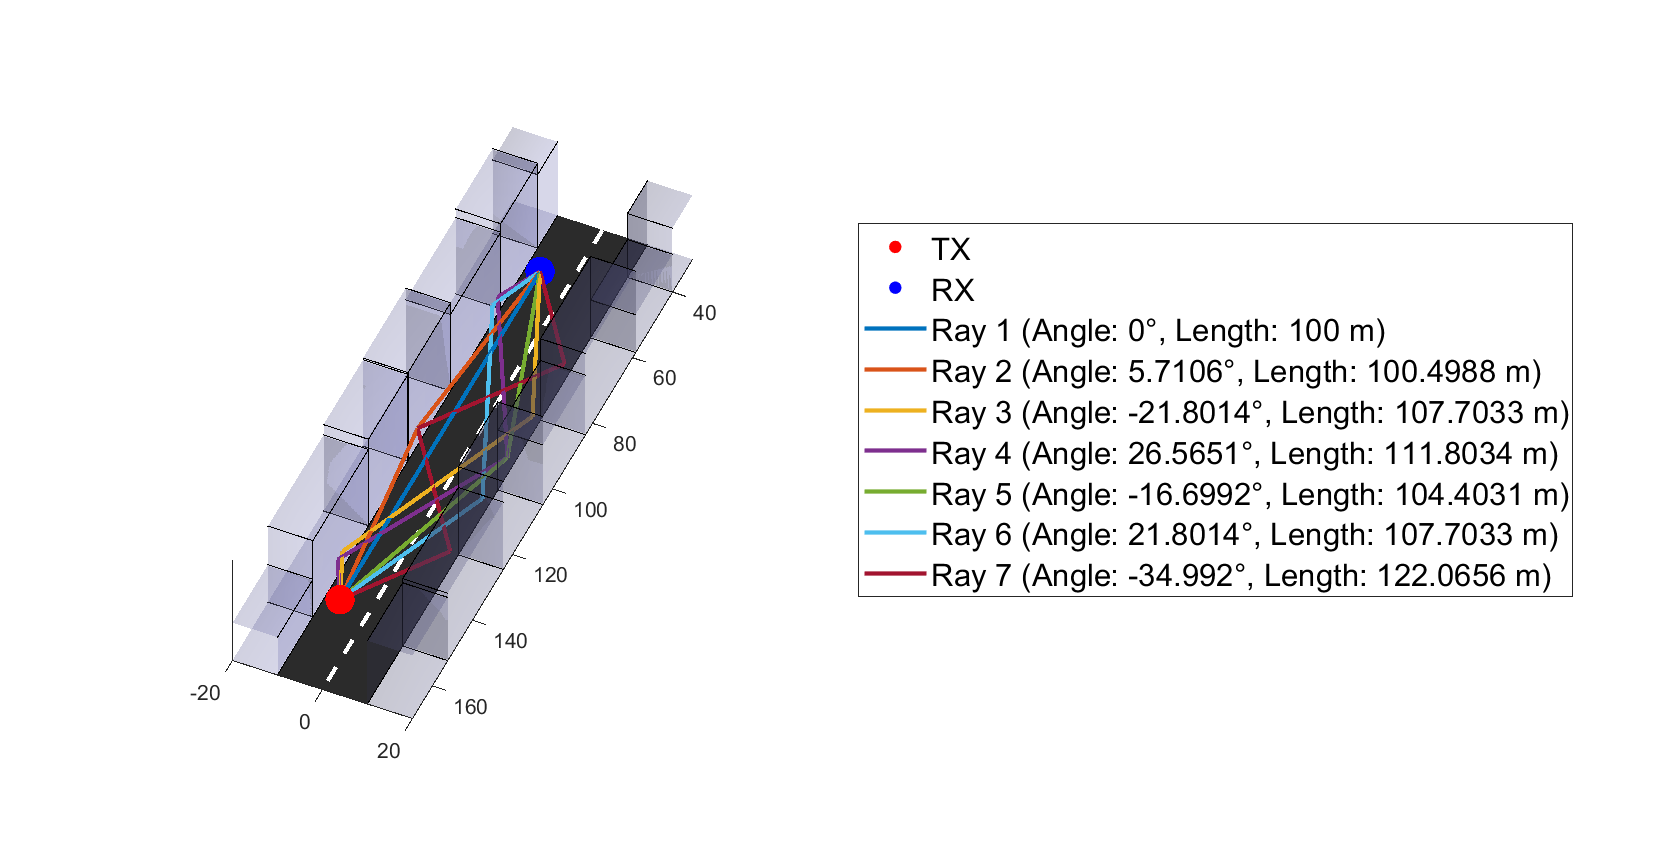
\includegraphics[width=1\textwidth]{3_1.eps}
    \caption{Raytracing simulation of a road surrounded by buildings}
    \label{fig:raytracingDemo}
\end{figure}

The received voltage has been computed on the same setup using equation \ref{eq:voltage_RX} to which the reflection coefficients $\Gamma_{\perp}$ have been added. 

\begin{align*}
    \Gamma_{\perp} = \frac{\cos \theta_i - \sqrt{\epsilon_r-\sin^2\theta_i}}{\cos \theta_i + \sqrt{\epsilon_r-\sin^2\theta_i}}
\end{align*}

The voltage carried by each ray is shown in figure \ref{fig:voltageDemo} using a colormap and the exact values are given in table \ref{tab:ray_properties}. The total received voltage is computing by summing the voltages of each ray and taking the phase into account. This gave the following result:

\begin{align*}
    \text{Total voltage} = 145.6 \mu V \angle -48.8^\circ
\end{align*}

\begin{table}[H]
    \centering
    \begin{tabular}{|c|c|c|c|c|}
        \hline
        Ray Index & Ray physical angle (°) & Ray length (m) & Carried voltage ($\mu V$) & Phase (°) \\ \hline
        1 & 180.0 & 100.0 & 129.1 & 30.0\\ \hline
        2 & 174.3 & 100.5 & 114.6 & -81.2\\ \hline
        3 & -163.3 & 104.4 & 88.9 & -3.7\\ \hline
        4 & -158.2 & 107.7 & 51.2 & -149.3\\ \hline
        5 & 158.2 & 107.7 & 51.2 & -149.3\\ \hline
        6 & 153.4 & 111.8 & 24.9 & 161.93\\ \hline
        7 & -145.0 & 122.1 & 15.0 & -134.1\\ \hline
    \end{tabular}
    \caption{Ray properties: index, angle, length, and voltage amplitude}
    \label{tab:ray_properties}
\end{table}

\begin{figure}[H]
    \centering
    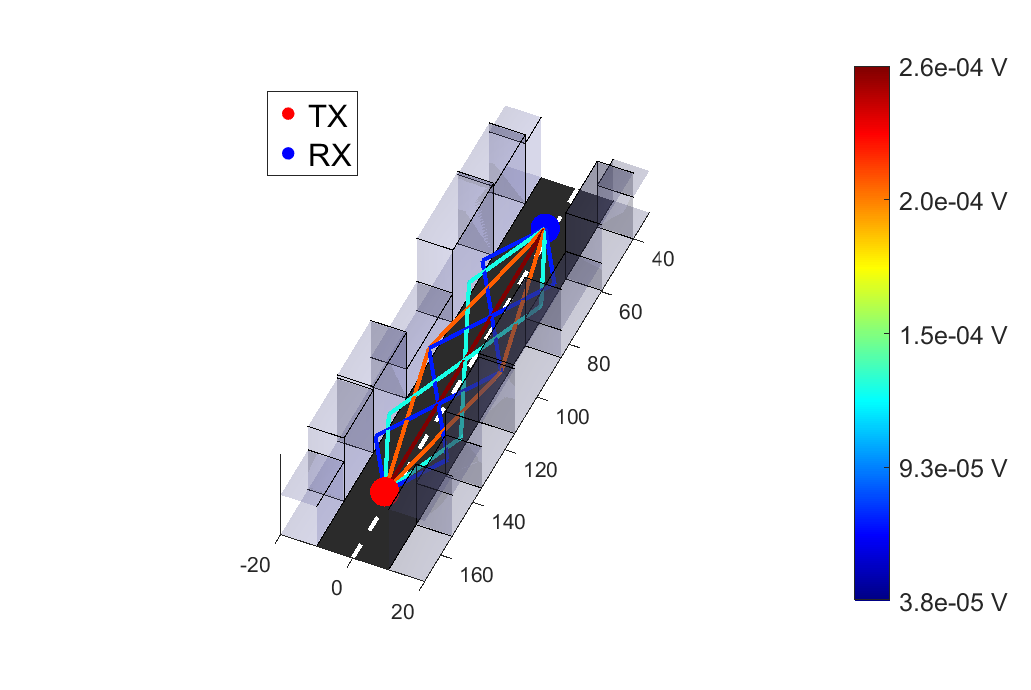
\includegraphics[width=0.8\textwidth]{3_2.eps}
    \caption{Received voltage for each ray}
    \label{fig:voltageDemo}
\end{figure}

By varying the distance between the two communicating cars between 0 and 1000m, a comparison is made between the raytracing simulation and the theoretical model on figure \ref{fig:P_RX(d)}. The simulated power is computed by taking the square of $V_{OC}$ divided by $Z_L \mathbin{\|} Z_a$ (see figure \ref{fig:equivalent_electrical_circuit}) and the theoretical power is computed using equation \ref{eq:power_friis_simplified}.

\begin{figure}[H]
    \centering
    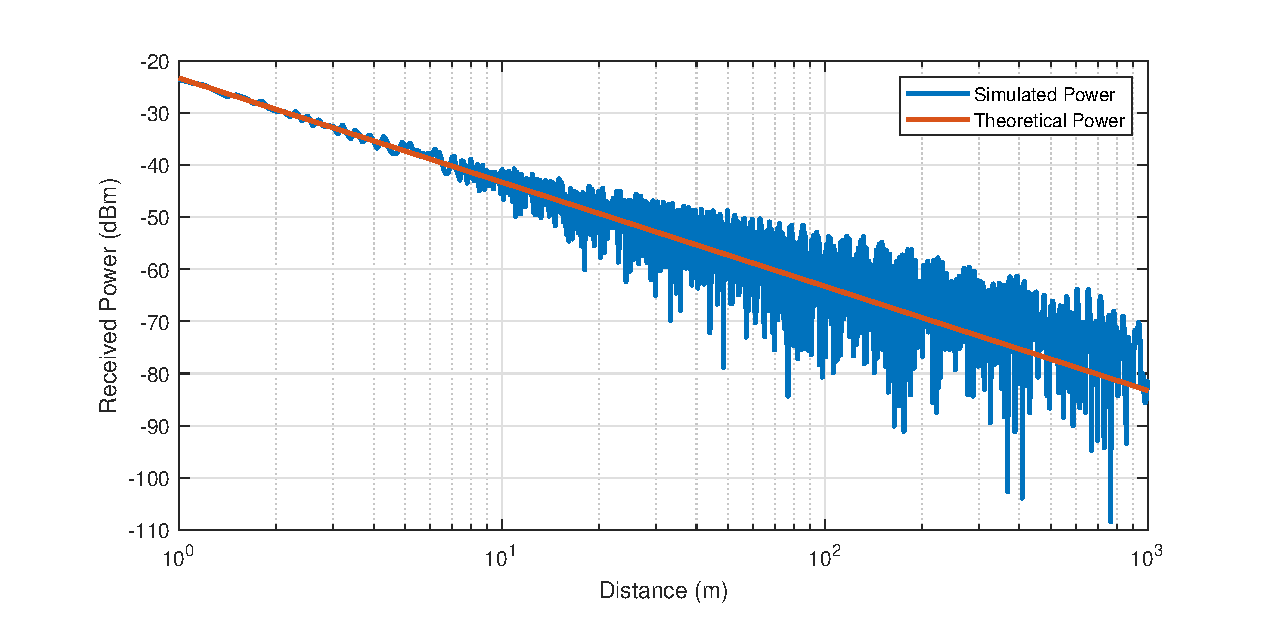
\includegraphics[width=1\textwidth]{3_3.eps}
    \caption{Received power as a function of the distance between the two cars}
    \label{fig:P_RX(d)}
\end{figure}

For short distances, the LOS ray is the only one contributing to the received power which explains the good match of the simulation with theory. \\
After a few meters, the multi path components (MPC) start to have an impact on the received power and the resulting interferences make the simulated power oscillate around the true power. \\
At greater distances and because of the limited number of bounces, one can clearly see the power is a multisine signal. This is because the reflection angles don't vary much with the distance at that point.\\

The oscillation around the expected power can be modeled with a Rice distribution as the LOS ray is the strongest one. The Rice factor $K$ is defined as the ratio between the power of the LOS ray and the power of the other rays:

\begin{align*}
    K = \frac{a_0^2}{\sum_{n=1}^{N}a_n^2}
\end{align*}

where $a_n$ is the amplitude of the $n^{th}$ ray with $a_0$ the amplitude of the LOS ray. As those amplitudes vary with distance, figure \ref{fig:K(d)} shows the rice factor as a function of the distance between the two cars. 

\begin{figure}[H]
    \centering
    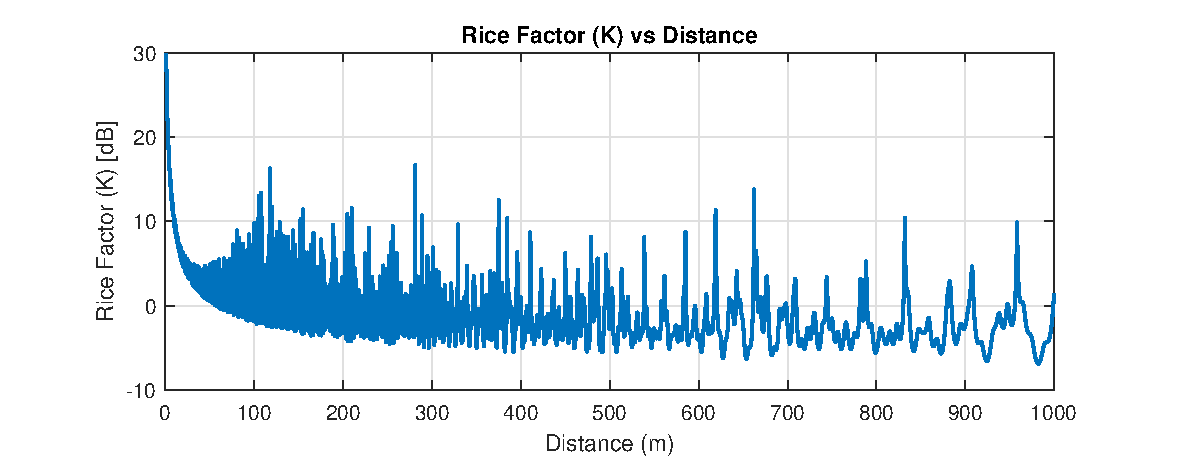
\includegraphics[width=1\textwidth]{3_4.eps}
    \caption{Rice factor as a function of the distance between the two cars}
    \label{fig:K(d)}
\end{figure}

The average received power in local areas is computed using:

\begin{align*}
    <P_{RX}> &= \frac{1}{8 Z_a} \sum_{n=1}^{N} \left| V_{OC} \right|^2\\
    &= \frac{1}{45\pi} \sum_{n=1}^{N} \left| V_{RX} \right|^2\\
\end{align*}

Where the sum is done over all the received rays. Figure \ref{fig:average_power} shows the average received power in local areas with a width of 5m for an emitter placed at the intersection of the two roads. The power is in dBm as it quicly becomes very small. \\
Another simulation has been done with 2m wide local areas and an emitter placed a bit further from the intersection. The result is shown in figure \ref{fig:average_power_2m} and it can be clearly seen that it is really difficult to get any power when no LOS ray is present. \\
It must be mentioned that the simulation does not take any transmission ray into account. This is under the hypothesis that the walls of the buildings are thick enough to not let any ray pass through.

\begin{figure}[H]
    \centering
    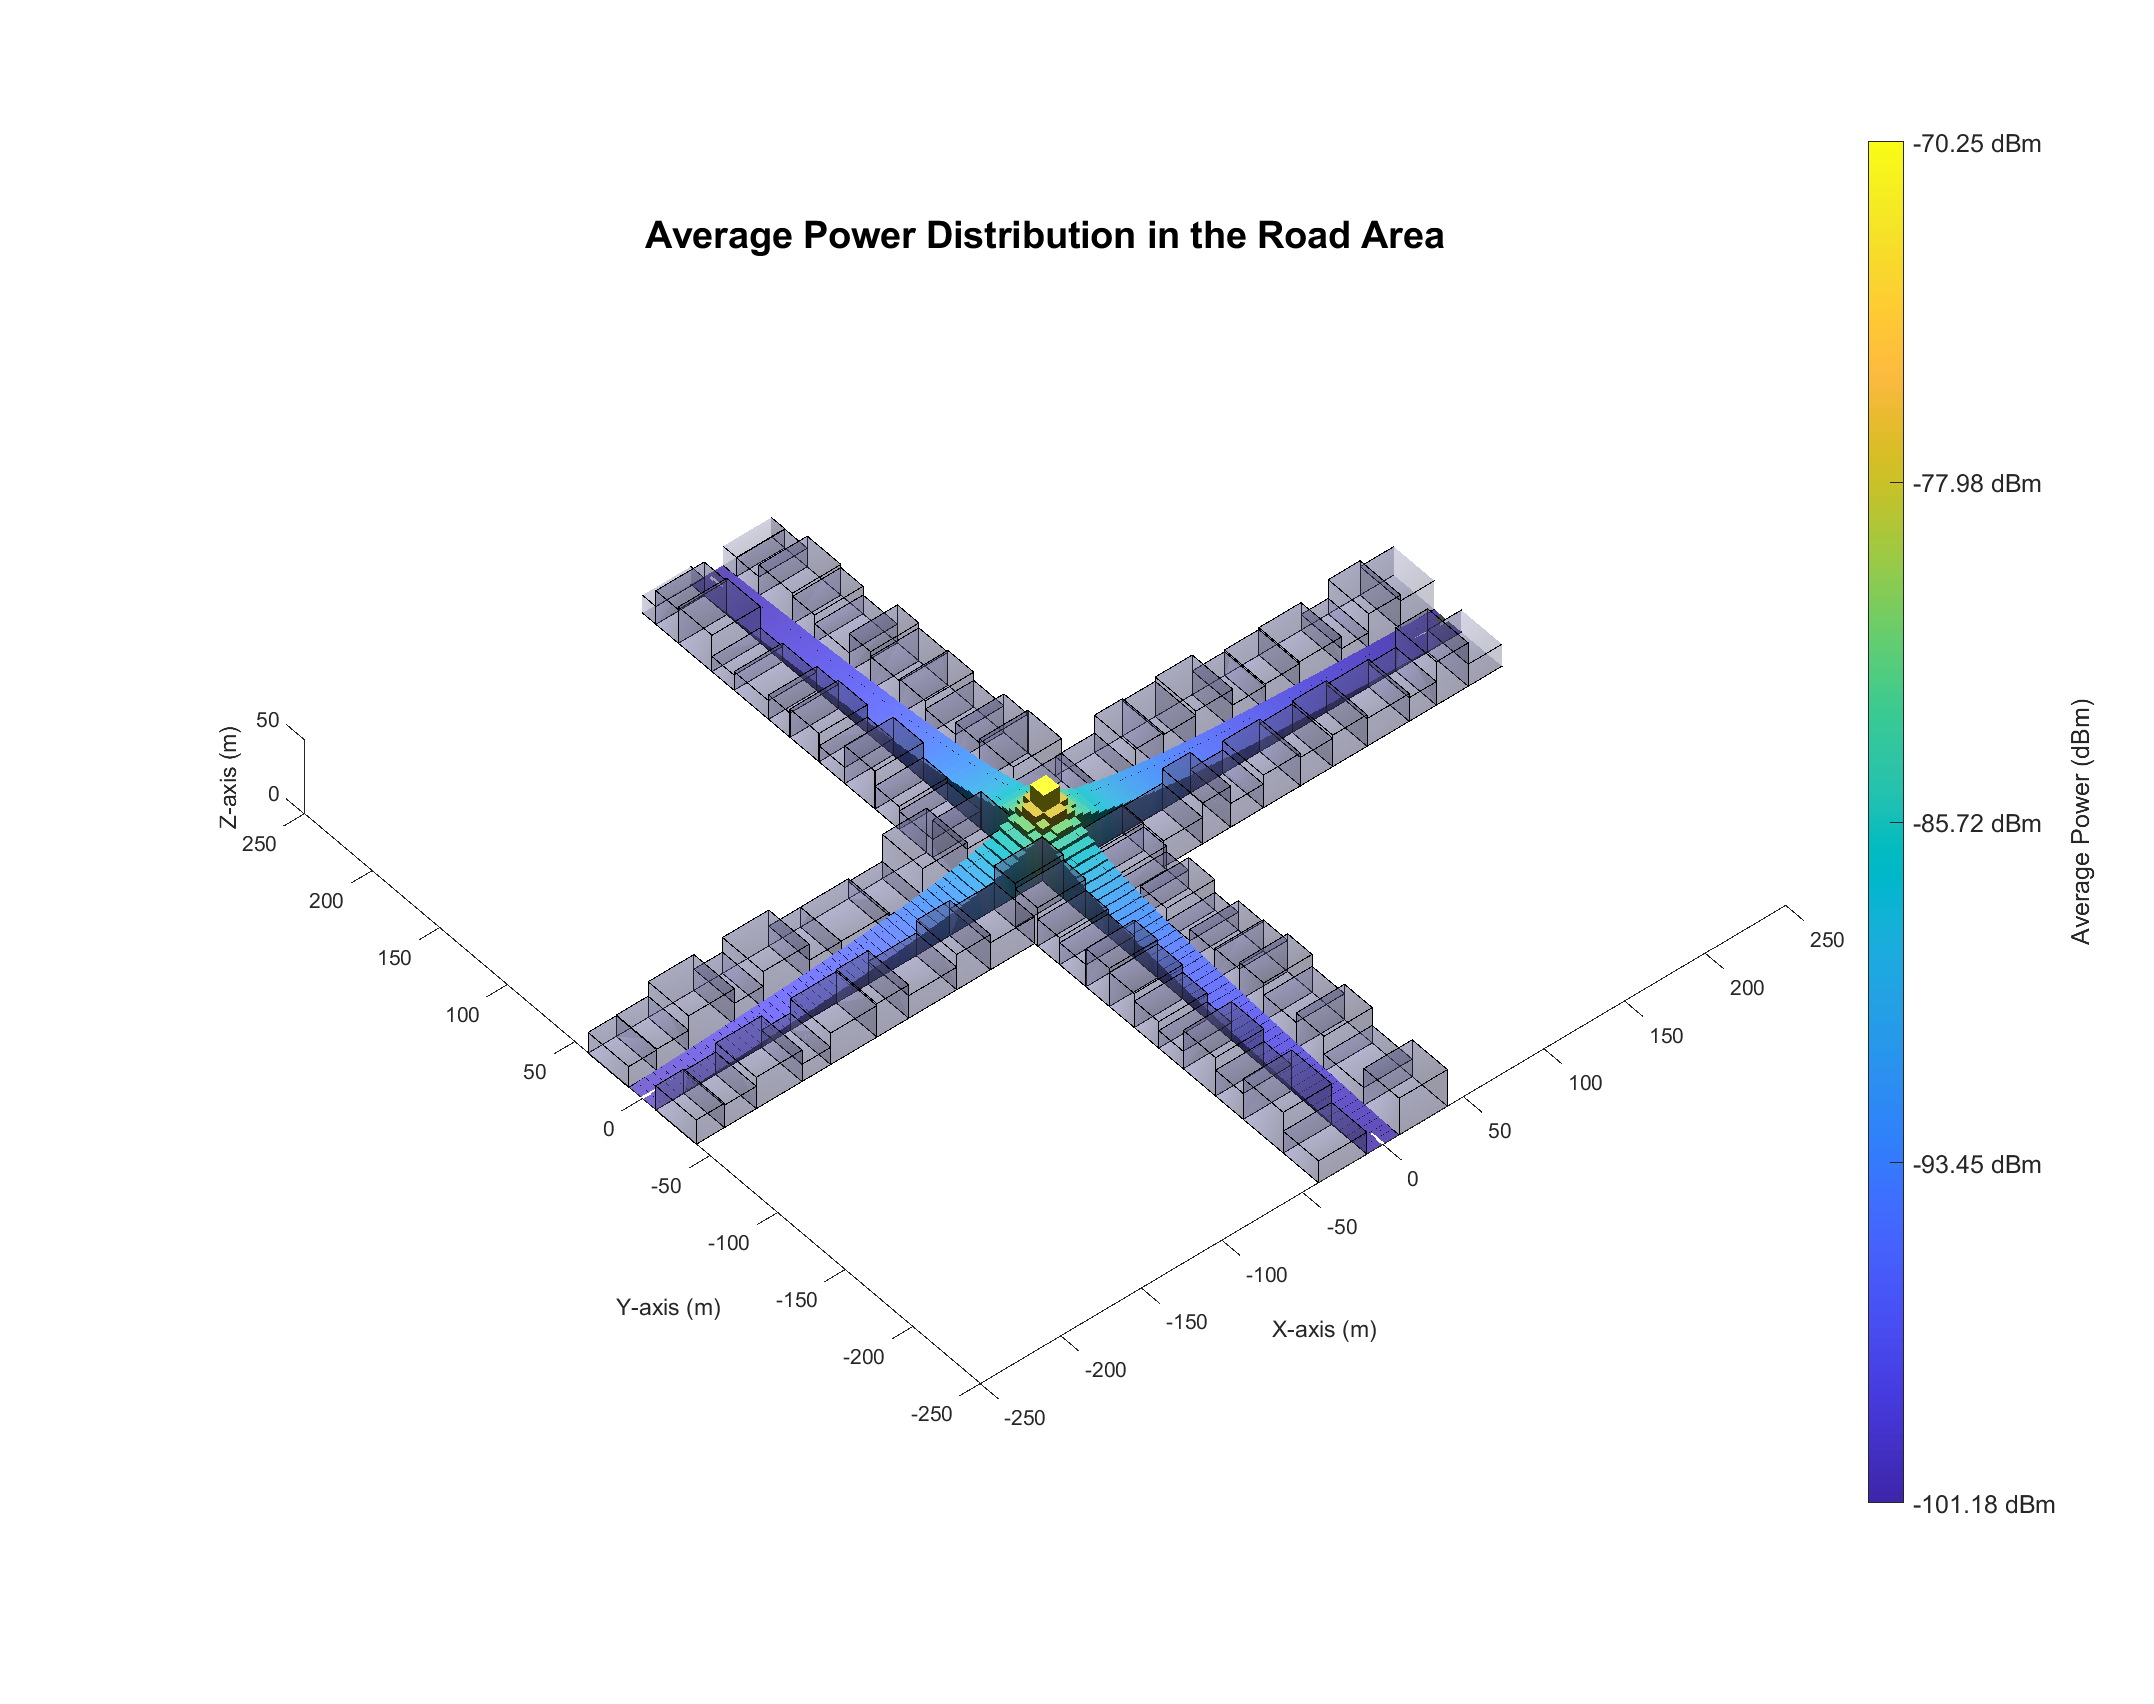
\includegraphics[width=1\textwidth]{3_5.eps}
    \caption{Average received power in local areas of 5m}
    \label{fig:average_power}
\end{figure}

\begin{figure}[H]
    \centering
    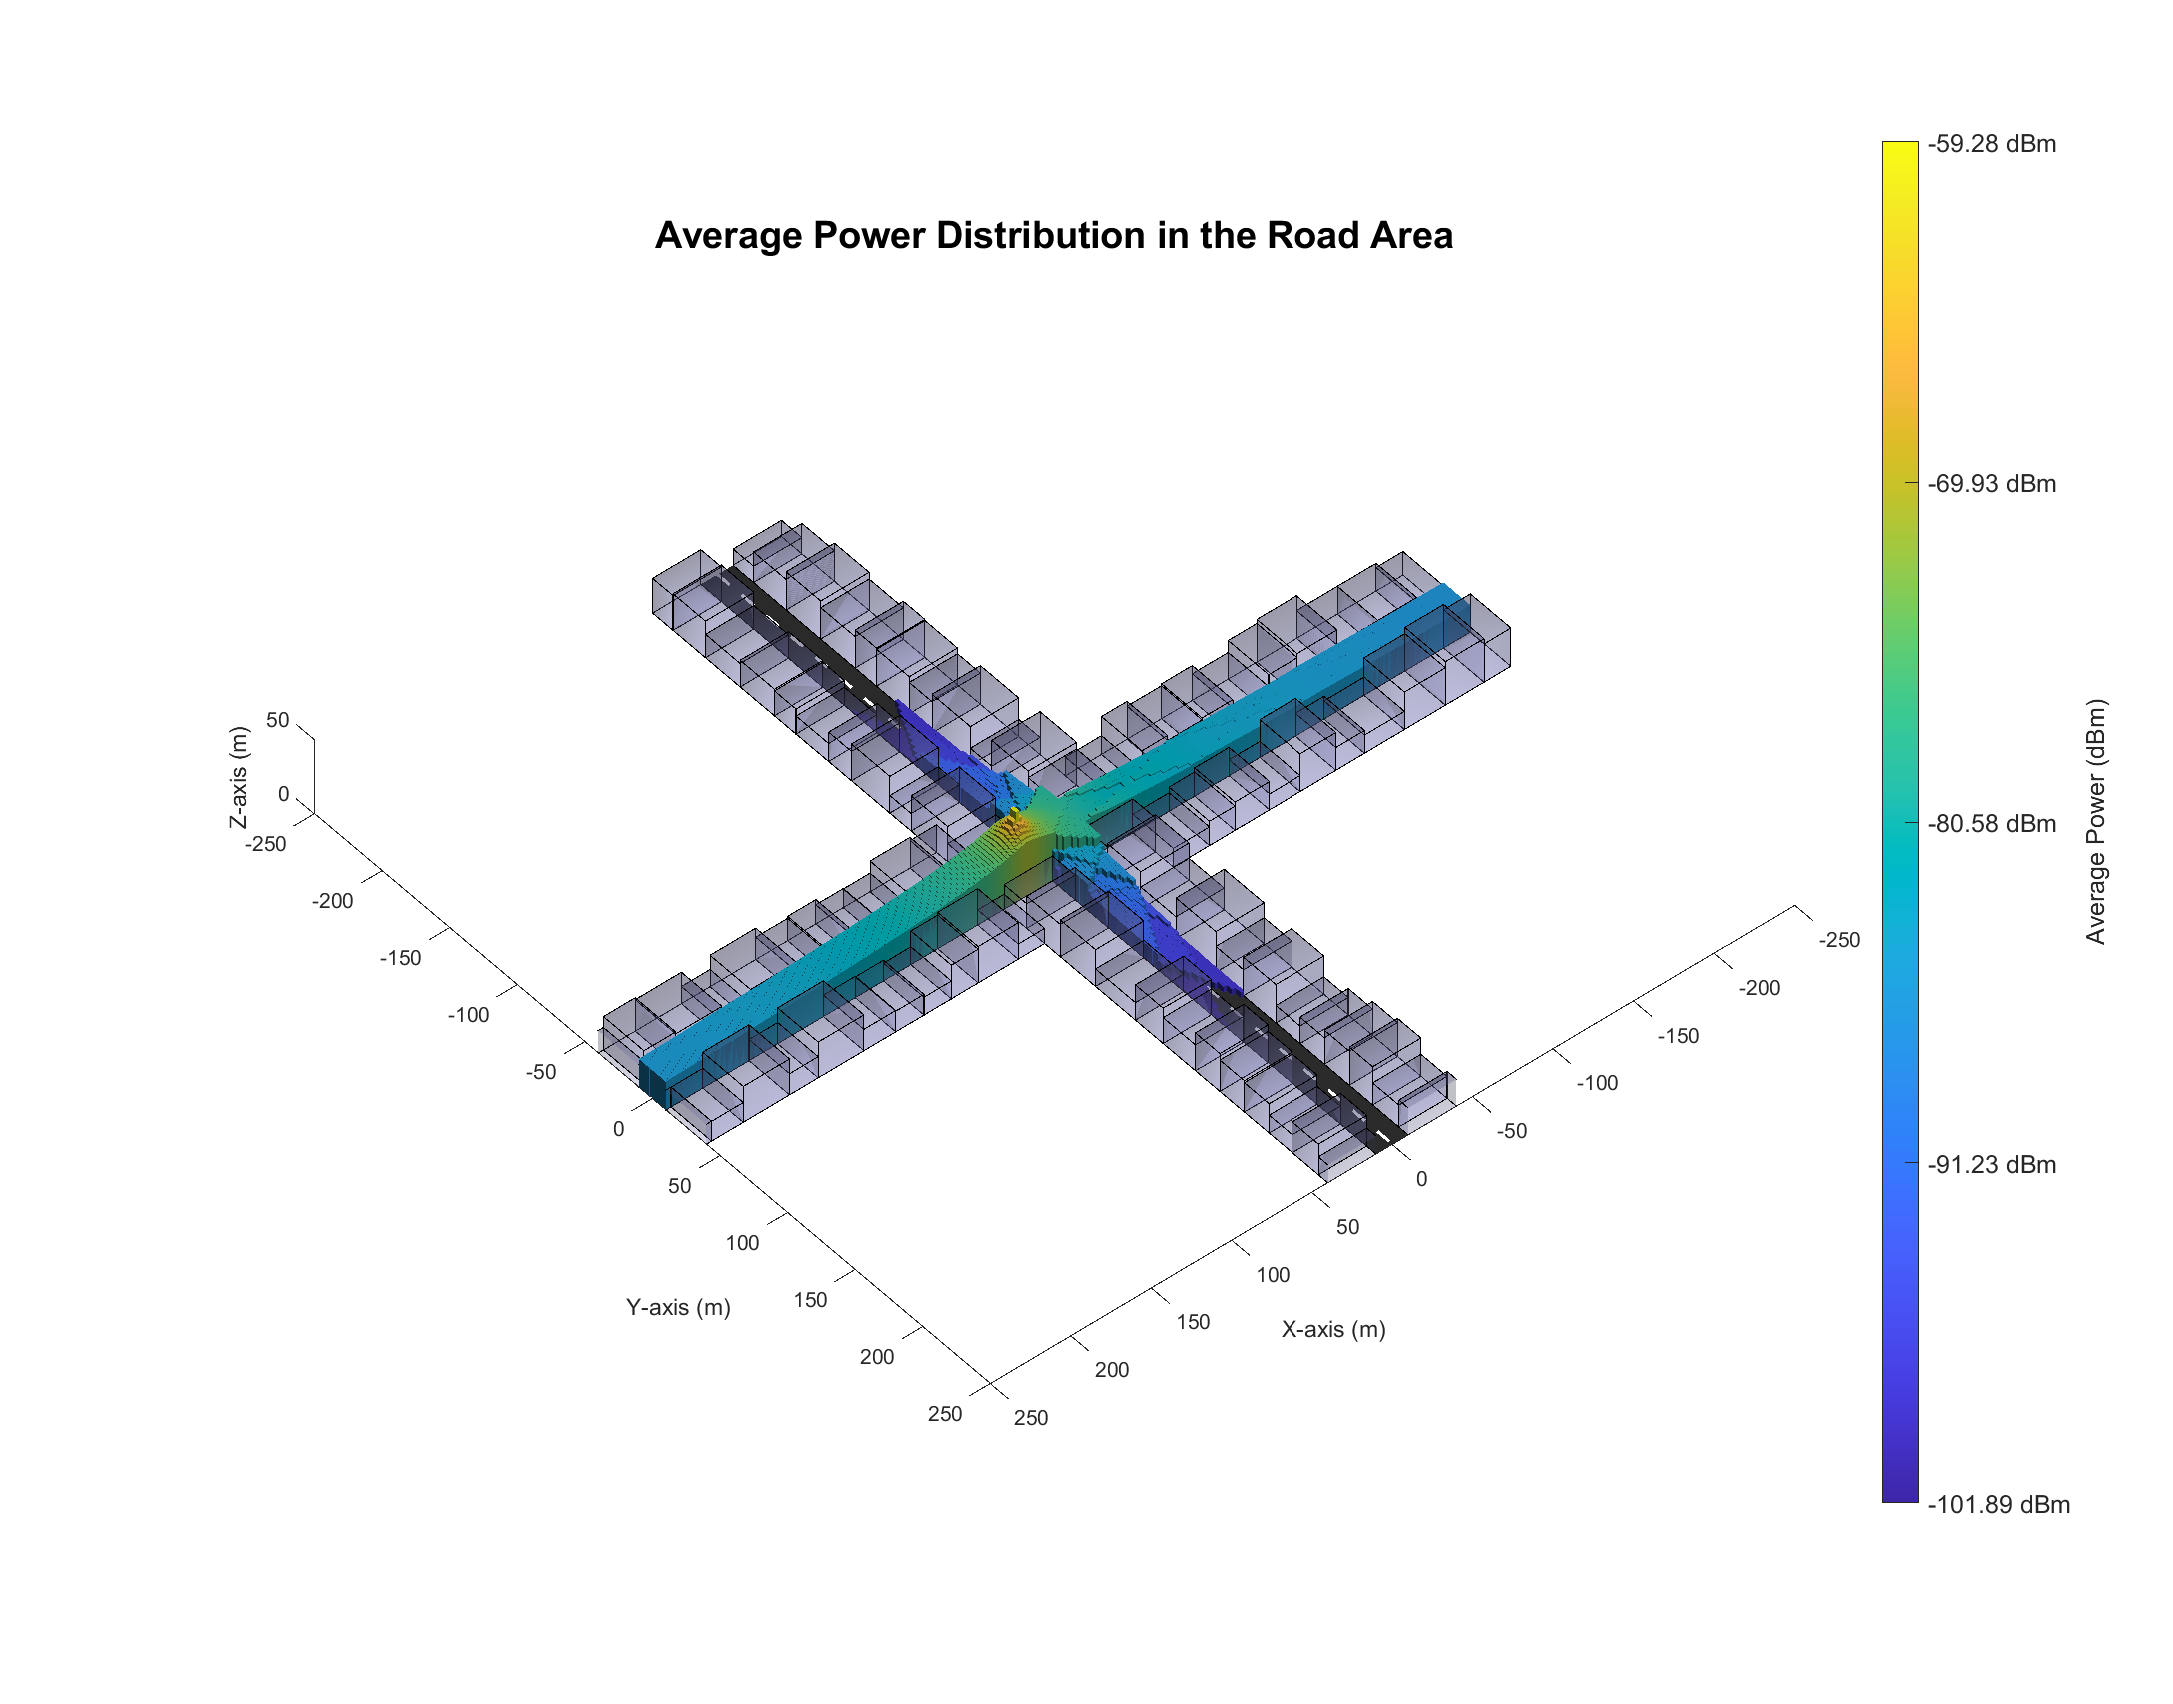
\includegraphics[width=1\textwidth]{3_5_alt.eps}
    \caption{Average received power in local areas of 2m}
    \label{fig:average_power_2m}
\end{figure}

The pass loss of the channel is defined (with every term in dB) as:

\begin{align*}
    L(d) = P_{TX} - P_{RX} 
\end{align*}

$L_0$ can then be defined as the pass loss that does not depend on the antennas. The canonical model for it is:

\begin{align*}
    L_0(d) &= L(d) + 10 log_{10} G_{TX} + 10 log_{10} G_{RX} \\
    &= L_0(d_0) + 10 n log_{10} \left(\frac{d}{d_0}\right)
\end{align*}

In which the parameters $L_0$ and $n$ must be found to fit the values of the simulation. $d_0$ has been arbitrarily set to 1m. The result is shown in figure \ref{fig:pass_loss} and the resulting parameters give as path loss model:

\begin{align*}
    L_0(d) = 58.501 + 10 \cdot 1.56 \cdot log_{10} \left(\frac{d}{1\text{m}}\right)
\end{align*}

\begin{figure}[H]
    \centering
    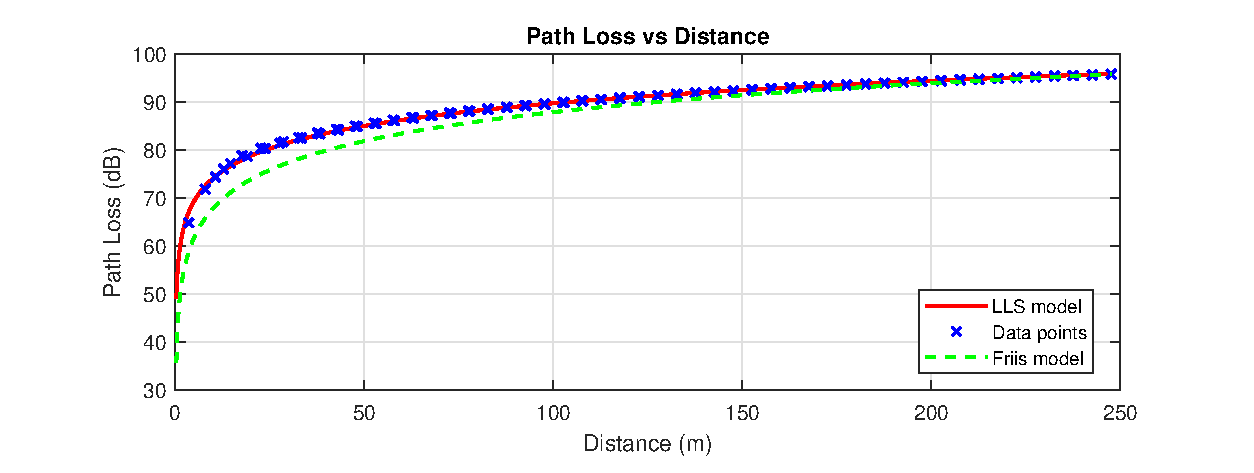
\includegraphics[width=1\textwidth]{3_5_model.eps}
    \caption{Pass loss of the channel and fitted model}
    \label{fig:pass_loss}
\end{figure}

As the LLS estimator only gives a "\textit{best fit}" to the data, there is still a parameter to define: the variability $\sigma_L$. It is the standard deviation of the path loss around the fitted model and its value here is:

\begin{align*}
    \sigma_L = 0.30236 \quad \text{dB}
\end{align*}

Regarding the communication reliability, it can be found under the assumption that the power variations due to shadowing is log-normal distributed. In this case, the probability of a successful communication is given by:

\begin{align*}
    \text{Pr} = \frac{1}{2} \text{erfc}\left(\frac{M}{\sigma_L}\sqrt{2}\right) 
\end{align*}

Where $M$ is the fade margin, defined as the difference between the received power and the minimum power needed to decode the signal. The fade margins required for a certain communication reliability are given in table \ref{tab:fade_margins}. They have been found by plotting the error probability as a function of the fade margin (see figure \ref{fig:fade_margin}).

\begin{table}[H]
    \centering
    \begin{tabular}{|c|c|c|}
        \hline
        Communication reliability & Fade margin (dB) & Cell range (m) \\ \hline
        50\% & 0 & \textbf{??}\\ \hline
        95\% & 0.4973 & \textbf{??}\\ \hline
        99\% & 0.7033 & \textbf{??}\\ \hline
    \end{tabular}
    \caption{Fade margins for different communication reliability}
    \label{tab:fade_margins}
\end{table}

\begin{figure}[H]
    \centering
    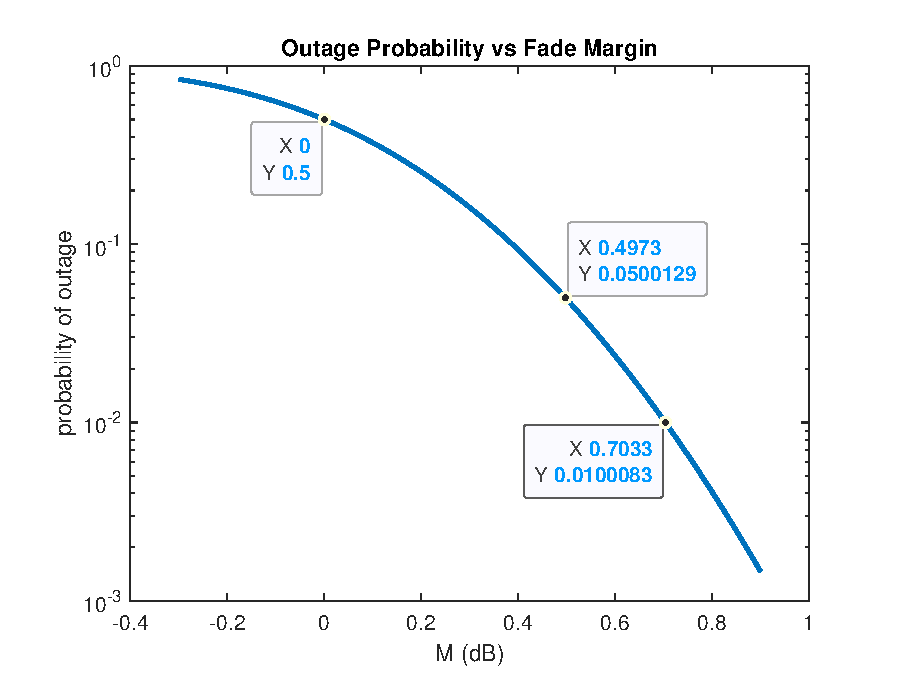
\includegraphics[width=1\textwidth]{3_7.eps}
    \caption{Fade margin as a function of the communication reliability}
    \label{fig:fade_margin}
\end{figure}

%\printglossary

%\printglossary[type=\acronymtype]

%Bibliography
%\nocite{*}
%\printbibliography[type=article,title=Articles]

\end{document}	
